\chapter{Backend} \label{backend}

Kód Backendu je rozdělen na dvě části, samotný Backend Mocasysu a
\\ \uv{DASCore}. DASCore poskytuje funkce pro řešení oprávnění přímo v
databázi a pro vytváření tzv. temporálních tabulek -- tabulek obsahujících i
historická data o každé změně.

Samotný Backend definuje tabulky systému a oprávnění nutná k jejich používání.
Tabulky jsou definovány standardní SQL syntaxí a pak jsou upraveny SQL funkcí.

Narozdíl od většiny systémů je vrstvám Mocasysu umožněn skoro přímý přístup k 
provádění SQL dotazů. Pro zajištění bezpečnosti bylo tak nutné implementovat
různá opatření přímo v databázi a využít tak pokročilé funkce PostgreSQL.

Při každém dotazu z Middleendu je vytvořeno spojení s databází a je spuštěna
funkce \texttt{session\_user\_set(user\_id, secret)}, kde \texttt{user\_id} je ID
uživatele získané z session tokenu a \texttt{secret} je klíč použitý k odhlášení
uživatele z daného databázového připojení a jeho navrácení do výchozího stavu.
Tato funkce, napsaná v jazyce Perl, uloží ID uživatele do globální proměnné pro
použití při ověřování práv.

Jednotlivé tabulky jsou pro potřeby uživatele databáze reprezentovány pomocí
\uv{views}, které mají nastavený atribut \texttt{security\_barrier}, což zakazuje
některé optimalizace a umožňuje tak použít \texttt{WHERE} klauzi k filtrování
tabulky dle oprávnění uživatele.

Omezení úprav je realizováno pomocí \texttt{INSTEAD OF} triggerů, které při
nedodržení podmínek zahlásí chybu a ukončí spojení.

Na verzované, temporální, tabulky je použito rozšíření PostgreSQL
\texttt{temporal\-\_tables} \citep[viz][]{TemporalTables} a pomocné funkce, které
k jedné tabulce vytvoří další pro ukládání historie a agregační view, které
zobrazí stav tabulky v globálně určeném čase.

Tato funkcionalita je obsažena ve funkcích, jejichž použití lze ukázat na
tabulce \texttt{food}:

\begin{code}
-- Vytvoří tabulku, ve které budou uložena data
CREATE TABLE IF NOT EXISTS food_current (
    id serial PRIMARY KEY,
    name text NOT NULL
);

-- Vytvoří tabulku pro ukládání historie a agregační view
SELECT version_table('food');

-- Stanoví nutná oprávnění k čtení a úpravám tabulky
SELECT dascore_setup_table('food',
    select_perm := $$ perm('food.select') $$,
    modify_perm := $$ perm('food.modify') $$);
\end{code}

\section{Databázové schéma}

Databázové schéma bylo navrženo obvyklými technikami jako jsou \uv{many-to-one} a 
\uv{many-to-many} vztahy a někdy i vztahem \uv{one-to-one}.
Bylo rozhodnuto, že se oddělí uživatel (tabulka \verb|users|),
strávník (tab. \verb|diners|) a osoba (tab. \verb|people|), 
což má několik důvodů. Ne každý uživatel musí být strávník.
Zároveň jedna osoba může mít více uživatelů, ale jeden uživatel
může mít k sobě přiřazeného pouze jednoho strávníka.
Příkladem budiž pracovník jídelny. Strávník může potenciálně být i třeba firma,
nebo jiný subjekt, takže je tak nechán prostor pro rozšíření.

Jak již bylo zmíněno, tabulky mají historii. Každá tabulka, kromě tabulky, která ukládá
data pro autentifikaci heslem, má suffix \emph{current} a párovou historickou tabulku,
která má suffix \emph{history}.

\paragraph{One to One}

\begin{itemize}
    \item users $\leftarrow$ user\_passwords\_data
    \item people $\leftarrow$ diners
\end{itemize}

\paragraph{One to Many}

\begin{itemize}
    \item people $\leftarrow$ users
    \item user\_mifare\_cards $\leftarrow$ users
    \item food $\leftarrow$ food\_assignments
    \item diner\_transactions $\leftarrow$ diners
\end{itemize}

\paragraph{Many to Many}

\begin{itemize}
    \item diners $\leftarrow$ food\_choice $\rightarrow$ food\_assignments
    \item users $\leftarrow$ user\_permissions $\rightarrow$ permissions
\end{itemize}

\noindent Na obrázku~\ref{dbSchema} můžeme vidět schéma s jednotlivými poli a jejich
datovými typy.

\begin{figure}
    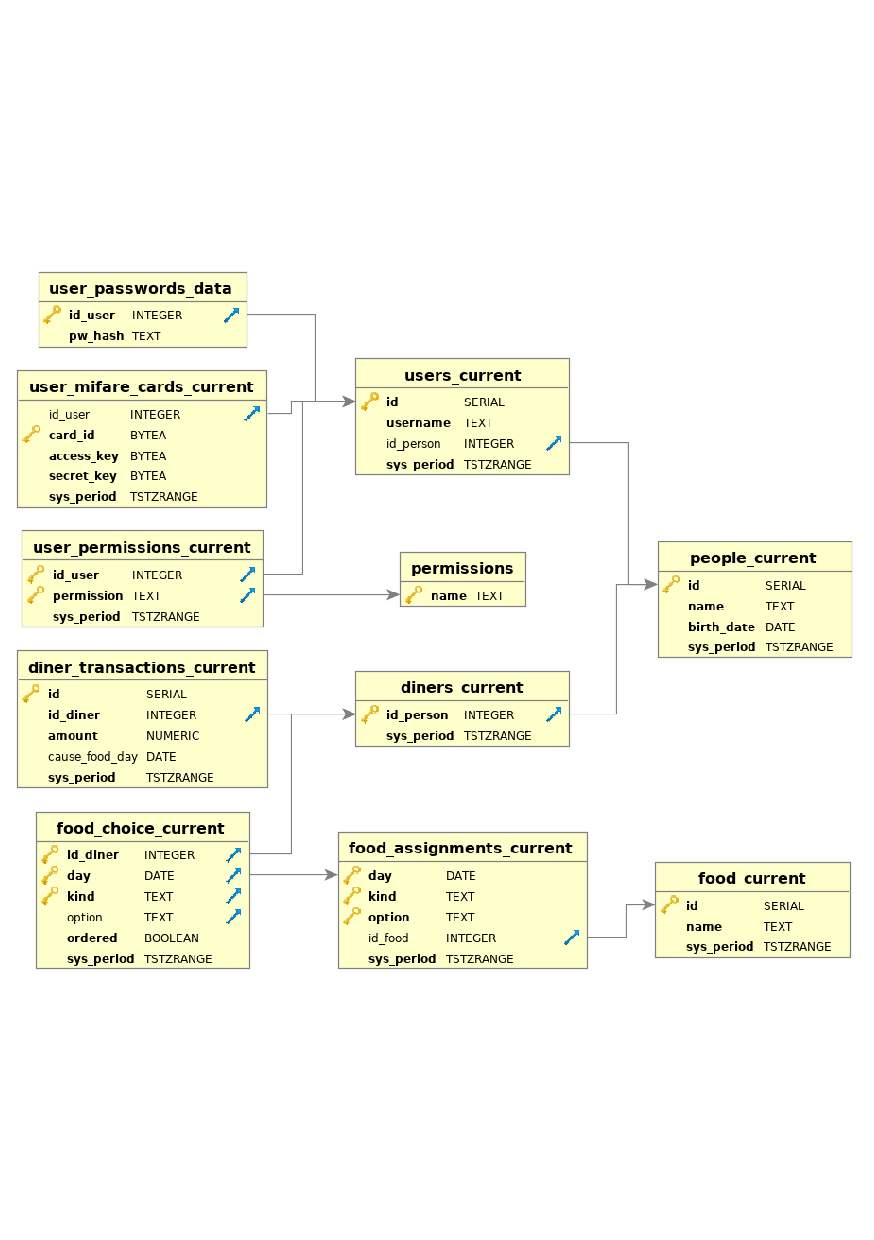
\includegraphics[width=140mm]{../img/db-schema}
    \caption{Databázové schéma. Vytvořeno programem DBVis.}
    \label{dbSchema}
\end{figure}
